%Intro_Arduino_ComputerControl
\chapter{Introduction to the Arduino}

\objectives{
\item Explain how to use a prototyping board, including the identification of
which pins are electrically connected.
\item Demostrate proper soldering technique.
\item Describe the two primary functions included in every Arduino sketch, when
they are called, and what they do.
\item Compile and upload sketches to an Arduino.
\item Demonstrate the use of digital output on the Arduino by constructing 
several circuits involving blinking lights.
}

\review{
\item Voltage (electric potential).
\item Current.
\item Resistance.
\item Diodes and LEDs.
}

There are two ways in which we want our computers to communicate with our
physics experiments:
\begin{enumerate}
\item Have the computer control the experiment. For example, we could have the
computer turn on our apparatus, or turn it off. 
\item Have the experimental device provide data to the computer. The computer
can then record this data for later analysis.
\end{enumerate}
In both cases, we need something that goes between the
experimental measuring devices and the computer. These go-between pieces are
often called Data Acquisition (DAQ) boards. There are many different forms
of DAQs. They can cost anywhere from a few dollars to many thousands of
dollars.

In this lab, we will use a low cost DAQ, the plans for which the 
developers placed in the open-source world so that no one
would get royalties (including themselves) for the design (this is why the
boards are inexpensive). It is low cost, but not low
quality. The developers named their DAQ the ``Arduino''. There are many
different variations on the Arduino. We will specifically be using the
Arduino UNO.

Like all DAQs, the Arduino is fragile, so we will need to exercise some 
caution. Arduinos can be destroyed by putting too large a voltage or electrical 
current into the input pins. They also can be destroyed by mechanical means, 
such as being dropped or crushed.








Let's start our study of computer control by controlling something simple
with our Arduino DAQ. Earlier we though about turning an apparatus on or
off. We can practice doing this with any device. While it might be exciting
to try this with a nuclear reactor, it will be easier (and safer!) to start
off simple. Let's turn on and off Light Emitting Diode (LED) lights.

\section{First Computer Control: LED blink (Step-by-step)}

Your instructor will provide you with a light emitting diode (LED) light, a
resistor, some wires, and a prototyping board. This last item helps hold the
other things in place so we can make electricity go through them. Here is
what we will build for our light blinking experience:

\begin{figure}[h!]
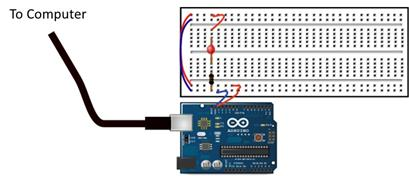
\includegraphics[width=3.4504in,height=1.4955in]{PH4CAU01}
\end{figure}You are probably familiar with
words like \textquotedblleft voltage\textquotedblright\ and
\textquotedblleft current\textquotedblright\ even though you have not yet
studied these in PH220. You have been plugging in things for many years now.
And so you know that \textquotedblleft voltage\textquotedblright\ has
something to do with electrical energy. That is enough for now. Our voltage
source is just a source of energy to make our circuits work.

A resistor is kind of what it sounds like. It tries to stop or slow down the
electricity in the circuit. The LED is just a circuit element that lights up
when electricity goes through it. You see them on computers and cell phones
as indicators that something has happened.

Let's assemble our system one step at a time.

\subsection{Prototyping boards}

Let's start with your prototyping board.

You might notice that the LED and the resistor in the diagram seems to be
stuck in some strange board full of holes. This is our prototyping board.
You should have one in your Arduino kit. Your instuctor will have several
that you can borrow if you need another one.

We will connect a lot of electrical wires together. We have devices to make
this job easier. Our porototyping board is one of these. They are officially
called prototyping boards, but you might hear them called proto-boards, or
even \textquotedblleft breadboards.\textquotedblright\ They are designed to
allow you to put an electronic element on the board and then connect other
things to that element. The boards look like this. \begin{figure}[h!]
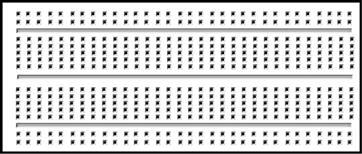
\includegraphics[width=3.0519in,height=%
1.3102in]{PH4CAU02}
\end{figure}

Notice that in the center of the board there are sets of five holes. Under
the board surface, these holes are connected together as shown by the red
lines in the next figure. \begin{figure}[h!]
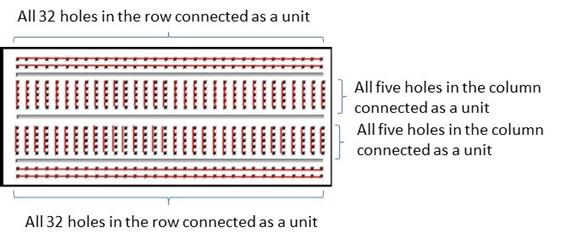
\includegraphics[width=4.8793in,height=2.0384in]{PH4CAU03}
\end{figure} Any wire that goes in one of the
connected holes is therefore connected to any other wire that goes in the
set of five connected holes. So you can connect up to four other wires to
the first wire. In the next figure, you can see an example of a resistor
that is placed on the proto-board and is connected to two yellow wires. 
\begin{figure}[h!]
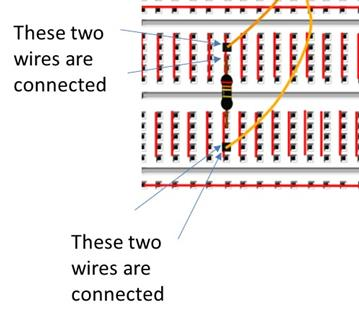
\includegraphics[width=3.0308in,height=2.6947in]{PH4CAU04}
\end{figure}Notice that each end of the
resistor is connected to a wire by placing the end of the resistor in one of
a set of five connected holes and by placing a wire in another of the set of
five connected holes. This would be a silly circuit to build. There is no
connection to a source of electrical energy. But this gives the idea of how
the prototyping board works.

There are also two long rows of holes on the side of the proto-board. These
are usually all connected along the whole row. \begin{figure}[h!]
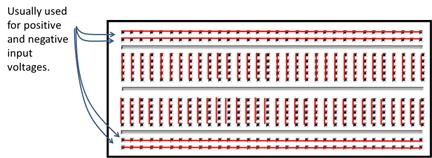
\includegraphics[width=3.6391in,height=%
1.3439in]{PH4CAU05}
\end{figure}Not all proto-boards are alike
when it comes to these long rows. But most are connected along the whole
row. These long rows are often used as a convenient way to make input power
available all along the whole board. Of course, once you know how the board
is wired underneath, you can use the connections any way that is consistant
with that design. We could skip using proto-boards and just connect
everything with wires and alligator clips. But proto-boards often make
holding everything in place much easier.

In today's lab experience, let's start by using the long rows as a place for
electrical energy to be used. We have long rows on the top and bottom of the
proto-board. For our first experience, we will use just $0\unit{V}$ and $+5%
\unit{V}.$ Let's make these voltages available on both the top and the
bottom of the board by wiring the two sets of rows together. \begin{figure}[h!]
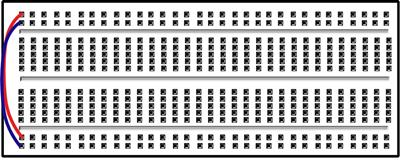
\includegraphics[width=%
3.3741in,height=1.3615in]{PH4CAU06}
\end{figure}%
Looking at our wiring diagram for the inside of the proto-board we can see
that how the top row and the second from the bottom row have been connected
with a wire (it is red if you are reading this in color) and the second from
the top and the bottom row are also wired together (the wire is blue if you
are seeing this in color). And we know that these entire rows are wired
underneath. \begin{figure}[h!]
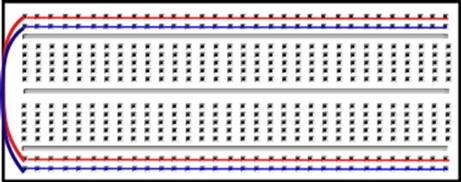
\includegraphics[width=3.4211in,height=1.3615in]{PH4CAU07}
\end{figure}Some proto-boards even have red
and blue lines to indicate that these rows can be used for electrical power.
Some of ours do.

Next let's add our LED light and our resistor. \begin{figure}[h!]
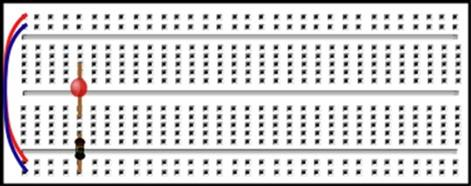
\includegraphics[width=3.9701in,height=%
1.5806in]{PH4CAU08}
\end{figure}Notice that the LED\ spans the
gap between the top and the bottom of the board.

In the next figure I have included our red connection lines so we can keep
in mind which parts of the proto-board are connected underneath.\begin{figure}[h!]
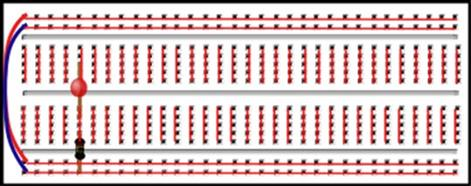
\includegraphics[width=3.9701in,height=1.5806in]{PH4CAU09}
\end{figure}

We placed one LED light wire in one column. On the other side of the board
we place the other wire. The wires that come out of an electronic device are
often called \textquotedblleft leads\textquotedblright\ and I will use this
term. So one LED lead goes in a group of five holes on one side of the board
and the other lead goes into a group of five hole on the other side of the
board. If you look closely, you will see that one side of your LED is flat.
The lead on the flat side should be toward the bottom (toward our $0\unit{V}$
connection that we will make). LED\ lights only work one direction. So when
using LED's, if they don't work, turn them around.

Notice that the way we have done this one LED lead and one resistor lead are
connected in one group of five holes. The resistor is connected to the very
bottom row. The top of the LED is not connected to anything yet. It is in a
set of five holes that are connected together, but we need another wire to
connect the top of the LED to the $+5\unit{V}.$ Let's choose the top of our
power rows to be $+5\unit{V}$ and add the wire to connect the LED. \begin{figure}[h!]
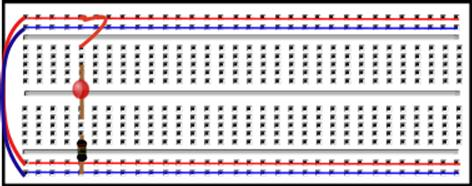
\includegraphics[width=3.979in,height=1.5806in]{PH4CAU0A}
\end{figure}

Now we can wire our light to our Arduino. This will take two wires. One
should be wired to pin13. The pin numbers are given on the side of the
wiring areas. \begin{figure}[h!]
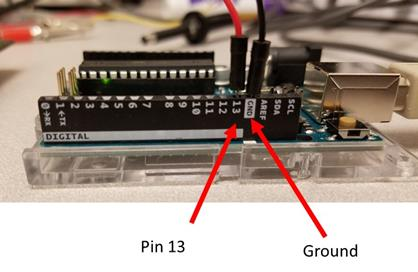
\includegraphics[width=3.5258in,height=2.3017in]{PH4CAU0B}
\end{figure}This pin 13 is a digital output.
That means it will either have $5\unit{V}$ or it will have $0\unit{V}.$ The $%
5\unit{V}$ will be our \textquotedblleft on\textquotedblright\ value that
could turn on an instrument. In our case it will turn on our LED\ light. The 
$0\unit{V}$ is the \textquotedblleft off\textquotedblright\ value. When pin
13 has a value of $0\unit{V}$ our light will go off. We know that voltage is
related to electrical energy. We will study voltage more next week. But for
now we need to know that voltage is a comparison. So we need to know
\textquotedblleft $5\unit{V}$ compared to what?\textquotedblright\ We
compare to the voltage of the ground. This is literal. Most buildings have a
large copper rod pounded into the ground. All of the plugs in the building
have one of their three wires connected to this rod. Thus they are all
\textquotedblleft grounded.\textquotedblright\ This is our reference. Our
computer is connected to a plug so it is grounded. Our Arduino is connected
to the computer so it is grounded. And one of our pins is a connection to
the ground. It is marked \textquotedblleft GND.\textquotedblright\ This will
be our $0\unit{V}.$ So we need to connect pin 13 and the GND pin to our $+5%
\unit{V}$ and our $0\unit{V}$ rows on our proto-board. The next figure shows
one way to do this.

\begin{figure}[h!]
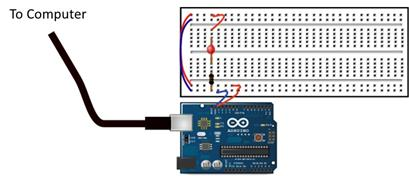
\includegraphics[width=3.4504in,height=1.4955in]{PH4CAU0C}
\end{figure}

We now have hour \textquotedblleft hardware\textquotedblright\ built for
blinking a light. But we need to give instructions to our Arduino that tells
it what to do with pin 13 and pin GND so our light will blink. Our Arduino
has a small computer on board, and we need a computer program to be uploaded
to the Arduino for this small computer to run. We will write and upload that
program next.

\subsection{LED light blink Sketch}

You wrote computer programs in Python in PH150. Our Arduino programs are
similar. They have loops and mathematical statements. There are some
differences as well. Our Arduino programs have special code
\textquotedblleft objects\textquotedblright\ for controlling our Arduino.
Most Arduino programs are very short. We just need instructions to tell the
Arduino what to turn on, turn off, or what data to collect. For today's lab,
we just need to address the digital output pins.

Let me introduce the commands we will use. Each digital output has a number.
The code defines a variable of type integer (int) and sets it equal to the
pin number. That pin can be HIGH or LOW with HIGH $=+5\unit{V}$ and LOW $=0%
\unit{V}$. Each digital pin needs to be set up for output or input. This is
done with a pinMode statement:

\begin{equation*}
\begin{tabular}{l}
pinMode(ledPin, OUTPUT)%
\end{tabular}%
\end{equation*}%
The variable ledPin is the pin number (for us 13). And the key word
\textquotedblleft OUTPUT\textquotedblright\ sets up our pin 13 to turn
things on or off.

To set the pin to HIGH use a digitalWrite command

\begin{equation*}
\begin{tabular}{l}
digitalWrite(ledPin,HIGH);%
\end{tabular}%
\end{equation*}%
and finally, to let the light be on for a while, use a delay command where
the delay time is given in milliseconds (ms)%
\begin{equation*}
\begin{tabular}{l}
delay(100);%
\end{tabular}%
\end{equation*}

These would not be normal Python commands. They are part of a specific code
library for use in making things with Arduino's.

We have a special development environment for programing our Arduino as
well. It looks like this. \begin{figure}[h!]
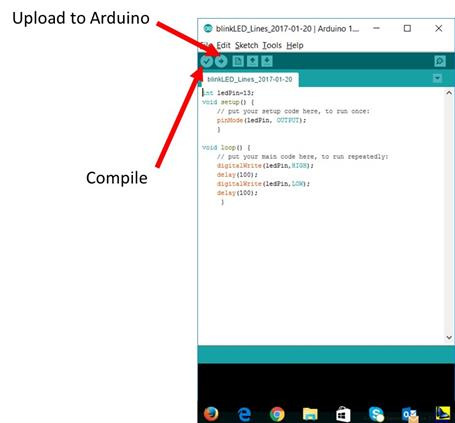
\includegraphics[width=3.8353in,height=3.5674in]{PH4CAU0D}
\end{figure}We will need to install this
development environment. To do so we go to
https://www.arduino.cc/en/Guide/HomePage and choose to instal the Arduino
IDE for your computer. IDE stands for \textquotedblleft integrated
development environment.\textquotedblright\ This is the environment that you
see in the last figure. It has two unusual buttons on its toolbar. One is
the \textquotedblleft compile\textquotedblright\ button. When you used
Python in PH150, you could run your code by pushing on a green arrow button
in most development environments. If you used Jupyter scripts, they also had
a function to run your code. But our Arduino is not big enough to be able to
run code this way. We need to convert our human-understandable code that
looks mostly like Python into a digital format that the Arduino can
understand. The compile button does this. As the code is converted, the
Arduino software looks for errors in the code. If there are errors, it will
tell you at this point. This is different than Python which only told you
about errors as the code ran. But remember we don't want to run our program
on our computer. We want it to run on our Arduino. So this check is good
before we send the translated code to the Arduino.

We also need a way to send our code to our Arduino and that is what the
upload to Arduino button does. Once the code is compiled without errors,
connect the USB\ cable to the Arduino and push the upload button.

There are also some syntax differences between the Arduino computer language
and Python. If you have taken CS124 or know the \textquotedblleft
C\textquotedblright\ language, you will recognize some of these changes.

\begin{itemize}
\item Everything in a function needs to be in curly braces \{ \}

\item Indenting is a good idea, but not required

\item comments can be started with two slashes //

\item every line needs a semicolon at the end;
\end{itemize}

\subsection{Arduino LED light blink sketch (program)}

We are ready to write code to blink our LED\ light. Here is an example code.
We write this code right in the Arduino development environment main window. You can download it directly \href{https://dtoliphant.github.io/PH250Manual/Code/IntroBlink.ino}{here}
\lstinputlisting[language=Arduino]{Code/IntroBlink.ino}


%\begin{lstlisting}[language=Arduino]
%/////////////////////////////////////////////////////////
%//Arduino Sketch to blink one LED light
%//   Written by Brother Lines
%//	(place your name here in your code)
%//   Feb 6, 2017
%//
%//   Define our Arduino Variables
%//      We will call pin 13 "ledPin"
%/////////////////////////////////////////////////////////
%int ledPin=13;
% 
%/////////////////////////////////////////////////////////
%// Arduino setup function comes next
%//    Every Arduino sketch needs a setup function
%//    We will set up our ledPin (pin 13) as an output pin
%void setup() {
% // put your setup code here, to run once to set up:
% pinMode(ledPin, OUTPUT);
% }
% 
%/////////////////////////////////////////////////////////
%// Arduino loop function
%//    Every Arduino sketch has a loop function
%//    This is where we put what we want the Arduino to do
%//    The Arduino will do whatever is in the loop function 
%//    until the Arduino is unplugged.
% 
%void loop() {
% // put your main code here, to run repeatedly:
% // turn on the LED
% digitalWrite(ledPin,HIGH);
% 
% // leave in on for 100ms
% delay(100);
% 
% // turn off the LED
% digitalWrite(ledPin,LOW);
% 
% // leave in off for 100ms
% delay(100);
% }
%/////////////////////////////////////////////////////////
%/////////////////////////////////////////////////////////
%\end{lstlisting}

Notice that we used a lot of comments. There are only ten lines that are
actually required to make the sketch run.

\begin{lstlisting}[language=Arduino] 
int ledPin=13;
void setup() {
 pinMode(ledPin, OUTPUT);
 }
void loop() {
 digitalWrite(ledPin,HIGH);
 delay(100);
 digitalWrite(ledPin,LOW);
 delay(100);
 }
 
\end{lstlisting}

The comments are not required for the sketch to work, but they help us
remember what we did later. In our class, \textbf{comments are required for
full credit}. So don't leave out the comments. In fact, you can add any
comments that might help you remember why the code works.

Also notice that Arduino programs are called \textquotedblleft
sketches.\textquotedblright\ Most of the commands are special Arduino
commands. And luckily, they make sense when we read them. Try it out. Type
in this sketch including the comments and compile and upload it to your
Arduino. If all goes well, the LED light will begin to blink. If all did go
well, go on to the next section. If it did not, call over an instructor.

Save your sketch and maybe take a photo of your hardware set up. Place both
in your lab notebook along with notes on how you got it to work. We will
build on this sketch, so spend some time documenting what you did in your
lab notebook so you can refer to it later.

\section{Second Computer Control: Two LED blink}

Now let's see if we can apply what we have learned. Let's change our
hardware so that it has two LED lights. Most of the hardware setup will be
the same. But We will wire them to two Arduino pins, say 12 and 13 (along
with GND of course) and have them blink, but blink independently.

We will have to abandon our nice $+5\unit{V}$ top row as our connection to
pin 13 because we need two pins, 12 and 13. The two pins must work
independently. In fact, let's have one LED\ on when the other is off.

This is why we can't wire both LED lights to the top row and wire the top
row to pin 13 as we did last time. That would make both lights blink at
once, but would not let one be off and the other on. Instead, let's wire the
top lead of one LED directly to pin 13 of our Arduino, and let's wire the
top lead of the other LED to pin 12. The two resistors can share a
connection to the GND pin, so let's keep using the $0\unit{V}$ bottom row of
the proto-board. Your hardware should look something like this.

\begin{figure}[h!]
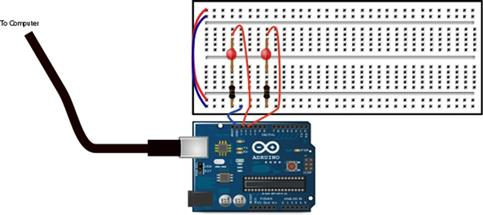
\includegraphics[width=4.0704in,height=1.8228in]{PH4CAU0E}
\end{figure}We will need to modify our sketch
(save the old one first so you have a separate copy for reference). Here is
a suggestion of what the new sketch might look like.

\lstinputlisting[language=Arduino]{Code/IntroBlink2LEDs.ino}


Again save your sketch and maybe take a photo of your hardware set up. Place
both in your lab notebook along with notes on how you got it to work. Make
sure others at your table are able to get their setup to work.

\section{Third Computer Control: Two LED blink using math}

Let's leave our hardware alone in the two LED setup from the last section.
And let's make the LED's blink the same way. But this time, let's calculate
when they should be on or off. Why would we do this? Because sometimes in
computer control of experiments we need to turn something on or off based on
a calculation. You may have your computer watching to make sure the
experiment doesn't get too hot or cold. The Arduino can bring in temperature
information, but you would have to write the code to tell it to turn off the
heater when your experiments gets to hot and to turn it on when it gets too
cold. This could be done with a mathematical comparison. We will use such a
comparison in the next sketch.

Suppose we want to know if a number is even or odd. Even numbers are evenly
divisible by $2.$ We could divide a number by $2$ and see if the remainder
is zero. Our Arduino language has a good set of mathematical functions. The
remainder function is a \textquotedblleft \%\textquotedblright\ sign. For
example 
\begin{eqnarray*}
3\%2 &=&1 \\
6\%2 &=&0
\end{eqnarray*}%
Let's have one light turn on if a number is even, then switch to the other
light if the number is odd.

In our code we will introduce a variable, $i,$ that we will increment (add
one to) every time the loop runs. So the first time the Arduino loop runs it
will be zero (even) and the next time 1 (odd) and the next time 2 (even) and
the next time 3 (odd) and so on. If you studied Python you would call such a
variable an \textquotedblleft integer\textquotedblright\ and might even know
to call it a \textquotedblleft loop counter.\textquotedblright

In our Arduino sketch we will test to see if $i$ is even in an if-statement.
If-statements go like this
 \begin{lstlisting}[language=Arduino]
 if (test condition ) {
   do something;
 }
 else {
   do something else;
 }
 \end{lstlisting}

Notice that the parts of the if-statement need curly braces. Our condition
to test is
 \begin{lstlisting}[language=Arduino]
i % 2 == 0
 \end{lstlisting}

Note that there are two equals signs. That makes it a test for equality
rather than an assignment. So we will have an if-statement like this
 \begin{lstlisting}[language=Arduino]
if (i % 2 == 0 ) {
 digitalWrite(ledPin1,HIGH);
 digitalWrite(ledPin2,LOW);
 delay(1000);
 }
 else {
 digitalWrite(ledPin1,LOW);
 digitalWrite(ledPin2,HIGH);
 delay(1000);
 }
 
 \end{lstlisting}

One last addition, our Arduino language has a shortcut for the statement
 \begin{lstlisting}[language=Arduino]
i=i+1
 \end{lstlisting}

It is simply
 \begin{lstlisting}[language=Arduino]
i++
 \end{lstlisting}

We will use this to make $i$ increase by one each time the loop runs. The
whole code might look like this.
\lstinputlisting[language=Arduino]{Code/IntroBlink2LEDs_Math.ino}



Again save your sketch. You should probably say in your lab notebook that
you used the previous hardware setup. You might want to describe in your lab
notebook how the mathematical algorithm works.

\section{Fourth Computer Control: Two LED blink in the Fibonacci sequence}

Suppose instead of LED\ lights we had large radio transmitters. And suppose
we were part of the Search for Extra-Terrestrial Intelligence (SETI). We
wish to send a message to any intelligent life that they would understand.
Intelligent life probably would be able to do mathematics and would
understand how mathematics occurs in nature. One sequence of numbers that
occurs over and over again in nature was discovered by Fibonacci. Let's
blink our LED\ lights (representing those powerful radio transmitters) in
the Fibonacci sequence.

We need to know now to calculate the Fibonacci sequence. One method is to
know that the sequence goes like this%
\begin{equation*}
0,1,1,2,3,5,8\ldots
\end{equation*}%
and that we can find the next number in the sequence by choosing $f_{1}=0$
first, then $f_{2}=1$ then using the formula 
\begin{equation*}
f(x-1)\ +\ f(x-2)
\end{equation*}%
Let's see that this works. For the first of the sequence, we just write the $%
0.$ For the second we just write the $1.$ Then for the third 
\begin{eqnarray*}
f_{3} &=&f_{2}+f_{1} \\
&=&1+0 \\
&=&1
\end{eqnarray*}%
So far so good. Let's try the next in the sequence%
\begin{eqnarray*}
f_{4} &=&f_{3}+f_{2} \\
&=&1+1 \\
&=&2
\end{eqnarray*}%
Again it worked. For the next one%
\begin{eqnarray*}
f_{5} &=&f_{4}+f_{3} \\
&=&2+1 \\
&=&3
\end{eqnarray*}%
and though we won't prove it, it works for every member of the sequence. See
if you can figure out how to write this code. An example is given below, but
see if you can figure out what the code should be.

This example is a much more complex version of a mathematical based computer
control.
\lstinputlisting[language=Arduino]{Code/IntroFibonacci.ino}
% \begin{lstlisting}[language=Arduino]
%/////////////////////////////////////////////////////////
%// code to blink two LED's using a mathematical expression
%// to determine when they should light. Note that the
%// Arduino code is closer to C++ than python.
%/////////////////////////////////////////////////////////
%int ledPin1=13;
%int ledPin2=12;
%int i=0; //loop counter
% 
%/////////////////////////////////////////////////////////
%int fib_count=0; // number of blinks based on Fibonacci
%int i_max=10; // maximum Fibonacci number before 
% // starting over
% 
%/////////////////////////////////////////////////////////
%void setup() {
% // put your setup code here, to run once:
% pinMode(ledPin1, OUTPUT);
% pinMode(ledPin2, OUTPUT);
% } 
% 
%int fib(int x) {
% // calculates the Fibonacci sequence using recursion
% if (x==0) 
%    return 0;
% if (x==1)
%   return 1;
%   return fib(x-1) + fib(x-2);
% } 
% 
%/////////////////////////////////////////////////////////
%void loop() {
% // put your main code here, to run repeatedly:
% // blink the LED's with the number of blinks being 
% // the Fibonacci sequence.
% fib_count=fib(i);
% if (i % 2 == 0 ) {
%   // turn off one light
%   digitalWrite(ledPin2,LOW);
%   // now blink the second light fib_count times 
%   for (int n=0; n<fib_count; n++) { 
%      digitalWrite(ledPin1,HIGH);
%      delay(100);
%      digitalWrite(ledPin1,LOW);
%      delay(100);
%   }
% }
% else {
%   // turn off the other light
%   digitalWrite(ledPin1,LOW);
%   // now blink the first light fib_count times
%   for (int n=0; n<fib_count ; n++) { 
%      digitalWrite(ledPin2,HIGH);
%      delay(100);
%      digitalWrite(ledPin2,LOW);
%      delay(100);
%   }
% }
% // increment i
% i++;
% // limit our blinks to the first i_max Fibonacci numbers
% if (i>i_max) i=0;
% }
%}
%/////////////////////////////////////////////////////////
%/////////////////////////////////////////////////////////
% \end{lstlisting}

Again save your sketch. You should probably say in your lab notebook that
you used the previous hardware setup. You really should describe in your lab
notebook how the mathematical algorithm works.

For next week, you should read the lab before coming to class. So your
assignment is to read Lab 2.

%TCIMACRO{\TeXButton{\vspace*{\fill}}{\vspace*{\fill}}}%
%BeginExpansion
\vspace*{\fill}%
%EndExpansion
\pagebreak
